\documentclass[conference]{IEEEtran}

\usepackage{cite}
\usepackage{amsmath,amssymb,amsfonts}
\usepackage{algorithmic}
\usepackage[brazil]{babel}
\usepackage[utf8]{inputenc}
\usepackage{graphicx}
\usepackage{textcomp}
\usepackage{xcolor}
\def\BibTeX{{\rm B\kern-.05em{\sc i\kern-.025em b}\kern-.08em
    T\kern-.1667em\lower.7ex\hbox{E}\kern-.125emX}}
\begin{document}

\title{Trabalho de Programação}
%----------------------------------------------------------------------------------------------------------
\author{\IEEEauthorblockN{Pablo Freitas Santos}
\IEEEauthorblockA{\textit{Engenharia Mecatrônica} \\
\textit{Univiversidade Federal de Santa Catarina}\\
Joinville, Brasil \\
pablo.santos1999@gmail.com}
}
%----------------------------------------------------------------------------------------------------------
\maketitle
%----------------------------------------------------------------------------------------------------------
\begin{abstract}

Esse trabalho Foi feito com intuito de implementar um algoritmo de uma telemetria partindo de um arquivo tabelado que lista dados de forma sequencial.

\end{abstract}
%----------------------------------------------------------------------------------------------------------

\begin{IEEEkeywords}
TDA, arquivos, estruturas
\end{IEEEkeywords}
%----------------------------------------------------------------------------------------------------------

\section{Introdução}

O cenário do esporte atual necessita de análise detalhada de cada informação captada durante uma partida, para isso foi preciso pensar em uma forma de listar todas as informações de cada jogador em um arquivo de acesso sequencial.

Nesse projeto foi utilizados tipos de dados abstratos, definido como  um conjunto de valores e uma sequência de operações sobre estes valores\cite{b1} para modularizar o código e aumentar a eficiência do sistema.

Com a utilização principalmente das TDAs, listas duplamente encadeadas e estrutura,  foram feitas operações com os dados obtidos, como por exemplo velocidade máxima, distância percorrida por cada jogador e tempo efetivo em campo. 

%----------------------------------------------------------------------------------------------------------
\section{Desenvolvimento}

A organização do trabalho foi feita em 3 partes: leitura do arquivo sequencial bruto e armazenamento dessa informação em uma lista duplamente encadear, seleção dos dados importantes a fim de fazer as operações e posteriormente a realização das operações previamente definidas com os dados convertidos

Primeiro, foi preciso utilizar meios de captação de linhas como fgets, na leitura do arquivo e colocar essa linha em forma de vetor de caracteres em uma lista sempre inserindo no próximo da cauda, mantendo todas as informações em ordem até encontrar o final do arquivo e retornar essa lista.

Em seguida, cada célula da lista retornada passou a conter uma linha do arquivo, mantendo uma ordem que facilite o uso de seus dados para os cálculos solicitados, como por exemplo, tempo local e velocidade. 

Para armazenar esse dado, foi criado uma lista cujos dados são outras listas, o que significa que cada célula da lista principal era uma sublista contendo as informações dos jogadores. Assim, foi possível acessar a informação de outro jogador independente da ordem que esse dado foi armazenado.

Além disso, foram consideradas informações após serem tratadas em uma estrutura chamada informação dos jogadores, possuindo a velocidade, identidade do jogador e  o tempo separado em horas, minutos, segundos.  

Antes de ir para a parte dos cálculos, foi pensado em uma forma de avaliar por período escolhido pelo usuário.

Assim foi criado uma entrada para definir previamente qual o tempo de cada parte do jogo que será tomado como parâmetro nas operações a serem avaliadas.

Nas operações, houve a utilização de um molde em todas as funções criadas , o qual foi feito na forma que a função recebe como parâmetro uma célula, que é referente da cabeça da lista do jogador em questão que foi armazenada as informações dos jogadores e foi utilizada para percorrer todos os dados que possuíam no seu interior. 

\begin{figure}[htb]
	\caption{\label{velmax}Exemplo do molde}
	\begin{center}
	    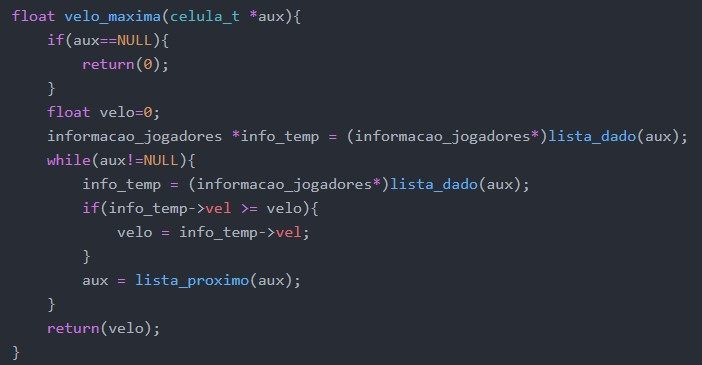
\includegraphics[scale=0.4]{figs/velo_max.jpg}
	\end{center}
	%\legend{Fonte:Elaborado pelo autor}
\end{figure}

Com isso, dependendo da informação requerida, foi utilizado um parâmetro de comparação para verificar a velocidade média atingida, por exemplo.

Um caso especial, foi a função que encontra quantas vezes o jogador ultrapassou a velocidade dada como parâmetro, foi implementada de forma recursiva, para exemplificar que pode ter outras formas sem ser a interativa de se revolver o mesmo problema e de forma mais compacta. 

\begin{figure}[htb]
	\caption{\label{Run}Ocorrências da velocidade dada como parâmetro}
	\begin{center}
	    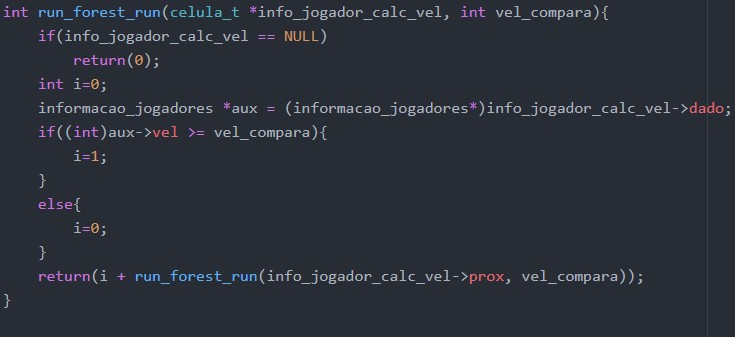
\includegraphics[scale=0.4]{figs/run.jpg}
	\end{center}
	%\legend{Fonte:Elaborado pelo autor}
\end{figure}

Foi utilizado a lógica de que quando  a função retornaria quantas vezes ele encontrasse o valor igual ou maior ao parâmetro, caso ele achasse algum que se enquadrava a essa condição era retornado a mesma função, mas dava um acréscimo de mais um e por fim quando chegasse no final dos dados ele retornava o valor final que era o objetivo da função.

Na parte de liberar memória alocada foi criado 3 funções de destruição: a de destruir lista por meio de recursão, destruir lista principal e destruir lista secundária. 

A divisão em etapas da destruição é importante porque a ordem em que o dado é liberado interfere no funcionamento correto do programa.

Além disso, como foi trabalhado listas que possuem em seu conteúdo outras sublistas então é uma solução modularizar a parte da destruição.



%----------------------------------------------------------------------------------------------------------
\section{Discussão}

O cenário do esporte atual necessita de análise detalhada de cada informação captada durante uma partida. Para isso foi de fundamental importância a utilização das TDAs para evitar erros e facilitar a identificar-los durante a construção do código, pois ao modularizar o código foi possível reutilização o mesmo e testar especificamente cada função.

Outro importante ponto foi utilização de listas duplamente encadeadas para acessar as informações guardadas nas estrutura. Como são listas pode-se acessar em qualquer lugar, mas nesse caso foi feito a utilização sempre em sequência do dado listado.

Chegou-se a resultados claros e definitivos apartir das informações dada pelo arquivo sequencial.

\begin{figure}[htb]
	\caption{\label{Resultado}Resultados}
	\begin{center}
	    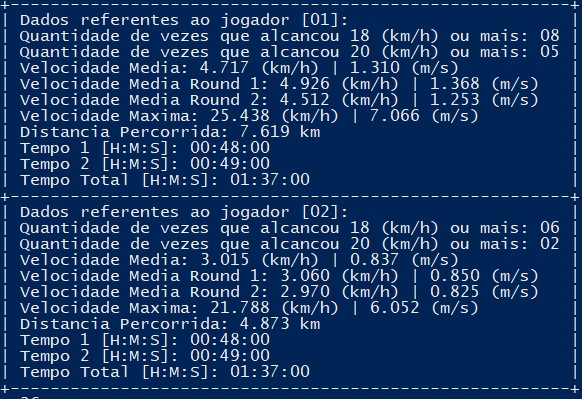
\includegraphics[scale=0.4]{figs/teste_csv.jpg}
	\end{center}
	%\legend{Fonte:Elaborado pelo autor}
\end{figure}

No entanto, houve problema com vazamento de memória devido à complexidade da manipulação dos dados. Para não comprometer as informações obtidas foram deixados alguns vazamentos no código.

\begin{figure}[htb]
	\caption{\label{Leak}Vazamento}
	\begin{center}
	    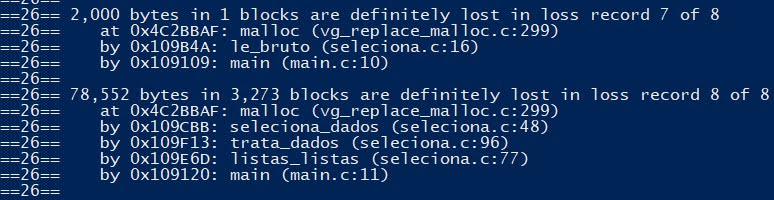
\includegraphics[scale=0.4]{figs/vazamento.jpg}
	\end{center}
    %\legend{Fonte:Elaborado pelo autor}
\end{figure}

No entanto, a maioria dos vazamentos apresentados possuem cerca de 24 bytes por bloco vazado, somente 1 não conseguiu ser destruído, pois é uma estrutura que armazena outra estrutura e para conciliar a integridade da informação e a memória não foi possível.

%-----------------------------------------------------------------------
\section{Conclusão}
Para construção de um algoritmo de captação de dados, é preciso se planejar na forma de organização desses dados e buscar separar-los por módulos de funções genéricas.

O planejamento desse código foi feito em função da necessidade da fácil mudança do algoritmo para buscar outras informações, listar todas as operações a serem feitas, para no momento de selecionar os dados coletar somente o essencial e deixar o código otimizado.

\begin{thebibliography}{00}

\bibitem{b1} TENENBAUM, Aaron M.; AUGENSTEIN, Moshe J.; LANGSAM, Yedidyah; SOUZA, Tereza Cristina Félix de. Estruturas de dados usando C. São Paulo: Makron Books, 2007. 426 p. (Programa do Livro Texto, 2007 ; 39). ISBN 8576051370
%\bibitem{b2} \url{https://www.geeksforgeeks.org/doubly-linked-list}


\end{thebibliography}

\end{document}
